%CREATED BY DAVID FRISK, 2016
\chapter{Methods}
This thesis is mainly experimental where more emphasis is put on the experiment 
rather than the theory. The process from start to finish consist of three main parts, the setup, 
the experiments and the data processing. The bare minimum of what was needed to conduct the experiment 
was a stage/arena to be the plane of motion, active and passive particles, and a recording contraption for collecting data. 
Since the scale of this experiment need to more or less resemble the simulation from \citeauthor{nilsson2017metastable}, 
it was clear early on that the arena of motion need to be relatively large, in comparison to the size of the particles. 
With a large stage, then there was the problem of capturing the whole stage. Also how should the active and passive particles 
be chosen? These issues will be addressed in the section below.

\section{The general experimental setup}

A opaque glass panel with dimension $\SI[product-units = single]{113 x 98}{\centi\metre}$ 
was chosen to be the surface of which the particles will move on. Glass was chosen for 
the reason that it ensures a hard and smooth surface, also it allows the option of 
filming the experiment from both above and below. To hold the glass panel tight and steady, 
a wooden frame was build in a way that allows the glass panel to be easily removed from, and 
put on to the wood construction. The finished glass table like construction is shown in \cref{fig:table}

\begin{figure}[htpb!]
    \centering
    %\captionsetup{justification=centering,margin=2cm}
    \includegraphics[width=.9\textwidth]
    {figure/equipments/table.png}
    \caption{A glass table construction where the experiments was conducted on. The construction including 
    the surrounding equipment consist of a main wooden frame with 4 table legs,  
    13 spotlights, a paper sheet, a glass panel, a boundary frame to prevent the particles from 
    falling from the glass, and a camera centered in the bottom of the table. As an example in this figure, 
    the active and passive particles are placed on the glass labeled as hexbug nano and obstacle, which 
    will be explained shortly.}
    \label{fig:table}
\end{figure}

\section{The boundary frame}

Note that \cref{fig:table} show the latest iteration of the setup with all its part. In previous iteration 
the boundary frame which was used for holding the particles inside the arena had a rectangular shape as 
in the right model of \cref{fig:boundary}.

\begin{figure}[htpb!]
    \centering
    %\captionsetup{justification=centering,margin=2cm}
    \includegraphics[width=.9\textwidth]
    {figure/equipments/boundary.png}
    \caption{The different boundary frame that were used, cloud shaped to the left and 
    rectangular to the right. The cloud shaped boundary(left) is an improvement from 
    the rectangular shaped one(right), with the purpose of redirecting the active particles 
    back to the center.}
    \label{fig:boundary}
\end{figure}

This rectangular shape turn out to be sub-optimal and lead to undesired behaviors with the active particles,  
where they often align with the walls of the frame and spend most of their time traversing alongside the boundary, see \cref{fig:walls}.


\begin{figure}[htpb!]
    \centering
    %\captionsetup{justification=centering,margin=2cm}
    \includegraphics[width=.6\textwidth]
    {figure/methods/20B491P2M_traj.png}
    \caption{A snapshot of an earlier experiment when the rectangular boundary was used. 
    The active particles tend to move alongside the walls of this boundary, as can be seen 
    from their trajectories(red lines) where it is more red at the four edges of the arena, 
    compared to the center.}
    \label{fig:walls}
\end{figure}

This sort of behavior was undesired since the particles did not interact much with on another and 
anything related to collective behavior was hard to see. The cloud shaped boundary was made to 
address this particular issue where the active particles now was redirected back towards center 
when hitting the wall, see left model in \cref{fig:boundary}.

\section{The active particles}

\subsection{The original robot bugs}

As for active particles in macroscale, toy robots called HEXBUG nano\textregistered\xspace were used, see \cref{fig:hexbug_nano}. 

\begin{figure}[htpb!]
    \centering
    %\captionsetup{justification=centering,margin=2cm}
    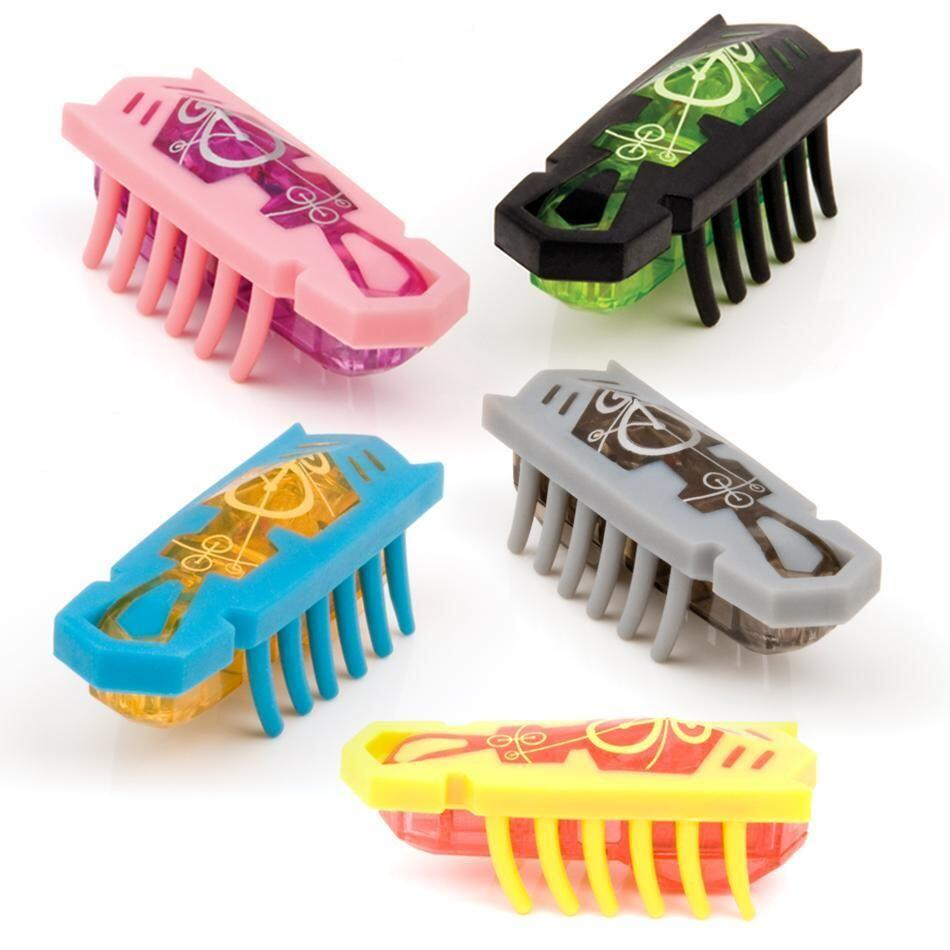
\includegraphics[width=.3\textwidth]
    {figure/equipments/hexbug_nano.jpeg}
    \caption{The commercialized toy robots HEXBUG nano\textregistered\xspace that were used as active particles in 
    macroscale, they have the dimension $\SI[product-units = single]{40 x 15 x 20}{\milli\metre}$ 
    and comes in many different colors, the image is copied from \cite{hexbug}.}
    \label{fig:hexbug_nano}
\end{figure}


This is just one of the many products by the company HEXBUG who is specialized in battery powered children's toy. 
The HEXBUG nano\textregistered\xspace is a micro robotic creature that uses vibration to propel forward. The vibration 
is powered by a tiny motor which in combination with the 12 angular legs is able to move the robot forward. The forward 
movement is a result of the robot legs being slightly bent backward compressing like a spring during the downward motion 
and then expanding converting elastic potential energy to kinetic energy pushing the robot forward, see \cref{fig:forward}.
The directional behavior of the bugs are random, while their velocity depend on the battery power which uses 
the type cell AG13/LR44 batteries. 

\begin{figure}[htpb!]
    \centering
    %\captionsetup{justification=centering,margin=2cm}
    \includegraphics[width=.5\textwidth]
    {figure/equipments/forward.png}
    \caption{A simplified scheme showing how the HEXBUG nano\textregistered\xspace are able to propel 
    themselves forward using only vibration from a motor and their legs which are tilted backwards.}
    \label{fig:forward}
\end{figure}


\subsection{Solar panel powered bugs}

In earlier stage of this project, there was an effort 
in trying to power the bugs using a solar panel. 
This was an effort in trying to minimize outside influences to the system, 
such as changing of batteries, also the intensity of illumination 
could be used as a parameter where it would affect the bugs activity.
The solar panel were placed on top of the bugs using 
lamps as source of illumination. In the first trial, 
a different type of commercial toy bug were used. 
These one was already made with solar panel built in, 
see \cref{fig:solarbugs}.


\begin{figure}[htpb!]
    \centering
    \subfloat[\label{fig:solarbugs}]
    {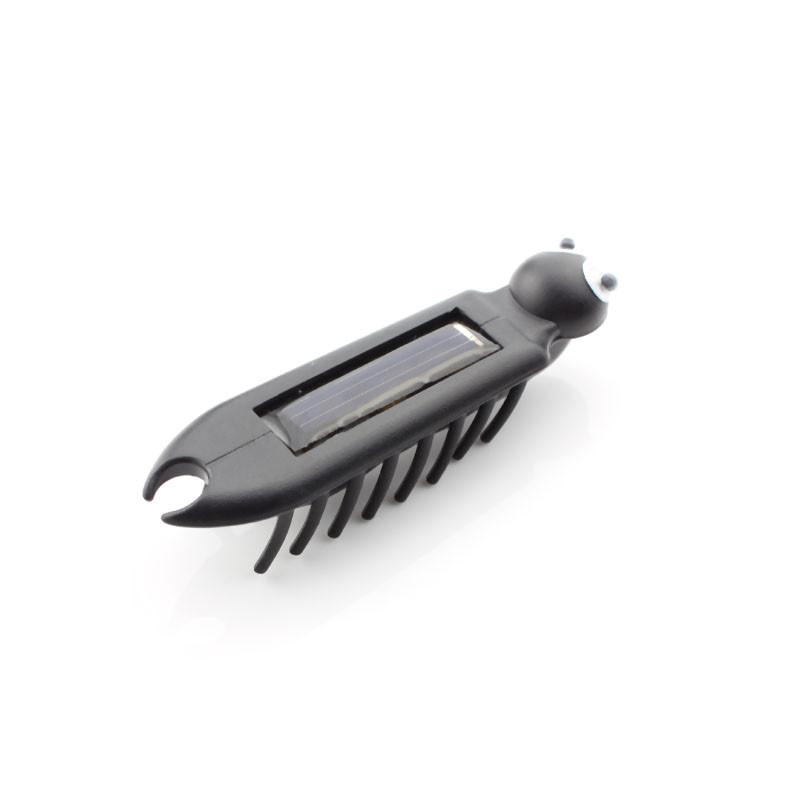
\includegraphics[width=.30\textwidth]
    {figure/equipments/solarbugs.jpg}}
    \subfloat[\label{fig:solarbugs_heat}]
    {\includegraphics[width=.45\textwidth]
    {figure/equipments/solarbugs_heat.png}}
    
    \caption{Toy solar bugs made in China in \textbf{(a)} with dimension $\SI[product-units = single]{60 x 15 x 12}{\milli\metre}$ 
    , the image is copied from \cite{www.alibaba.com}. In \textbf{(b)} is an experiment using these bugs with 2 construction 
    spotlights as light source.}
    \label{fig:solarbugs_experiment}
\end{figure}

These bugs were much less vibrant then the HEXBUG nano and required the light source to be very close 
to them. Also, they seem to only react on the type of light source that produces a large amount of heat, see \cref{fig:solarbugs_heat}, 
which over time does damage on the bugs. Being exposed to heat from lamps, the body of these bugs started to melt and there legs 
detached from the body as a result from the glue, connecting the legs to the body, melting. 

Having the practical issues mentioned above, the solar bugs were replaced with the HEXBUG nano, now with the battery removed and 
a solar panel mounted on top of the bug, see \cref{fig:hexbug_solar}.

\begin{figure}[htpb!]
    \centering
    %\captionsetup{justification=centering,margin=2cm}
    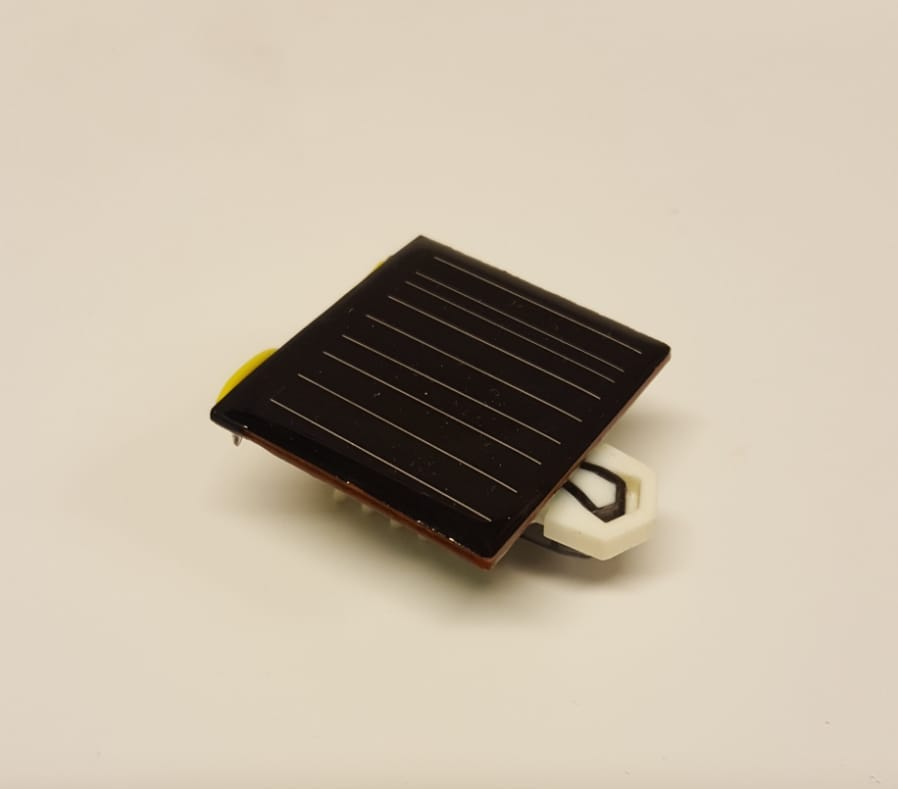
\includegraphics[width=.3\textwidth]
    {figure/equipments/hexbug_solar.jpg}
    \caption{The HEXBUG nano\textregistered\xspace with a solar panel mounted on top. The battery 
    inside the bug was removed and instead there are wires connecting the solar panel to the motor inside.}
    \label{fig:hexbug_solar}
\end{figure}

This arrangement with the solar panel on the HEXBUG, in \cref{fig:hexbug_solar} improved the motions of the bugs 
marginally. The bugs shows more activity compared to the Chinese made ones, but the extra weight 
and the rectangular geometry of the solar panel created some unwanted behaviors. The extra weight from 
the solar panel made the bug top heavy which caused them to sometimes tip over, and also if the panel 
was not centered on the bug well enough, the movement will be biased either left or right. The size of 
the solar panel with the dimension $\SI[product-units = single]{35 x 39}{\milli\metre}$ created unwanted 
contact interactions between the bugs such as the scenario where the solar panels from 2 different bugs would overlap 
and cling on to each other. With all this being said, the problem of illumination still remains where the illumination is 
still being too low and inhomogeneous, causing the bugs to move much slower than they would with battery and the 
speed was rarely constant.

Having all the practical issues mentioned before, the solar powered concept was abandoned and the project proceeded 
on using the original HEXBUG nano with battery, though with other minor modifications.

\subsection{The battery powered bugs}

As mentioned before, these bugs runs on type cell AG13/LR44 batteries, and can be used up to 4 hours before 
the battery need to be changed. When letting these bugs run on an empty arena, without passive particles, 
the bug show some random chirality(a tendency to move to the left or right) resulting in them moving in circles with 
the radius decreasing over time as the battery gets lower, see \cref{fig:chirality}. This chirality is probably a result of some asymmetry 
with the bug that appears during manufacturing.

\begin{figure}[htpb!]
    \centering
    %\captionsetup{justification=centering,margin=2cm}
    \includegraphics[width=.5\textwidth]
    {figure/methods/0W0C2B_traj.png}
    \caption{An experiment with 2 bugs with only one being tracked 
    with the red line showing its trajectory. The tracked bug was 
    running for approximately six seconds and has almost managed to 
    complete two full circles, which is a result of its chirality.}
    \label{fig:chirality}
\end{figure}

This chiral behavior is inherent to the bugs and different bugs has different degrees of chirality which 
cannot be predicted in beforehand. Though this behavior seems substantial, it can be neglected when 
the passive particles are introduced where collision-based interactions is dominated and the free running 
space is minimal.

\subsection{The shape of the bugs}

When using a new fully charged battery on a bug, their activity becomes quite vibrant. This lead
sometimes to them tipping up side down ending up on their back or climbing on top of each other. 
Even the shape of their head caused some unwanted behavior. The pointy shape of their head resulted oftentimes
in them being blocked between heavy obstacles, trying to push for a long time instead of finding a new path in 
other directions, see \cref{fig:stuck}.

\begin{figure}[htpb!]
    \centering
    %\captionsetup{justification=centering,margin=2cm}
    \includegraphics[width=.5\textwidth]
    {figure/equipments/stuck_V2.png}
    \caption{To the left is an example scenario where the robot bug is trying to push through heavy obstacles, for a long time 
    instead of finding a new path. To the right is the desired behavior where the bug first tries to push through the obstacles 
    but is unable to, it then changes its direction and finds new path.}
    \label{fig:stuck}
\end{figure}

The behavior of pushing through obstacles was not entirely unwanted since it was still necessary for
the bugs to create channels by pushing the obstacles. However, with the pointy heads, they tend to 
spend the majority of their time pushing i.e creating channels instead of reusing them, which makes 
it hard to observe any phase transitions or the reusing of channels.

Two new modifications were made to address this problem, see \cref{fig:shape}.

\begin{figure}[htpb!]
    \centering
    \subfloat[\label{fig:circle}]
    {\includegraphics[width=.45\textwidth]
    {figure/equipments/hexbug_cicle.png}}
    \subfloat[\label{fig:paper}]
    {\includegraphics[width=.45\textwidth]
    {figure/equipments/hexbug_paper.png}}
    \caption{Modified versions of HEXBUG nano, 3D printed plastic circle on the head in \textbf{(a)}, and 
    strip of paper wrapped around its body in \textbf{(b)}.}
    \label{fig:shape}
\end{figure}

The first attempt was to glue a piece of plastic circle on the bugs head as in \cref{fig:circle}, this way 
the bugs would have a better chance of bouncing away from the obstacles instead of spending too much time trying to push through them. 
However when using many bugs there was a problem of the circle head overlapping each other and become stuck, upon a collision. 
These unpredictable behavior required further improvements resulting in the latest version seen in \cref{fig:paper}. 

This modification here was rather simple using only a strip of paper to wrap around the bugs body. 
Compared to the previous versions, this modification does not add any significant weight to the original 
bug since the weight of the paper strip is neglectable compared to the weight of the bug. Also the weight 
is evenly distributed around the bug which will not amplify the bugs inherent chirality further. 
This rod shape is quite common in the field of active matter, presenting in theoretical models\cite{peruani2008individual}, 
Janus particles\cite{paxton2004catalytic}, and bacterias\cite{berg2008coli}, and furthermore 
the rod shape creates aligning interactions, see \cref{fig:align}, which is advantageous for the emergence of collective behaviors.

\begin{figure}[htpb!]
    \centering
    %\captionsetup{justification=centering,margin=2cm}
    \includegraphics[width=.4\textwidth]
    {figure/equipments/align.png}
    \caption{An example of aligning interactions between two rod shaped bugs upon collision.}
    \label{fig:align}
\end{figure}

With all the advantages mentioned, only the rod shaped bugs will be used to produce the results presented in this thesis.
For future reference, the terms active particles, robot bugs or bugs will be used interchangeably, referring to 
the Hexbug nano wrapped in paper strip.

\section{The passive particles}

The passive particles that were use to make up the complex environment are 3D printed plastic cylinder see \cref{fig:obstacle}. 
These cups are approximately $\SI{19.5}{mm}$ in diameter, $\SI{20}{mm}$ in height and weighs $\SI{2}{g}$.

\begin{figure}[htpb!]
    \centering
    %\captionsetup{justification=centering,margin=2cm}
    \includegraphics[width=.7\textwidth]
    {figure/equipments/obstacle.png}
    \caption{3D printed plastic cylinders(left) used as macroscale passive particles, made hollow in the 
    middle for the purpose of varying its weight by putting M8 nuts(right) in them. The cylinder 
    have dimensions $\SI[product-units = single]{19.5 x 20}{\milli\metre}$(radius $\times$ height) and 
    weigh $\SI{2}{g}$ each. The M8 nuts weigh $\SI{5}{g}$ each and only 3 nuts can be put in one cylinder.}
    \label{fig:obstacle}
\end{figure}

To vary the weight of each cylinder, M8 nuts were used to be placed inside the cylinders. The nuts weigh 
$\SI{5}{g}$ each, and each cylinder can hold up to three nuts. The possible weight that one cylinder can 
have is $\SI{2}{g}$(empty), $\SI{7}{g}$(1 nut), $\SI{12}{g}$(2 nuts) and $\SI{17}{g}$(3 nuts).
From this point on, for the sake of clarity, the term obstacle and passive particle will be used 
interchangeably.

%each and has a hole where weight can be added to them. The weight used are M8 nuts of $\SI{5e-3}{kg}$ each. 
%The number of these plastic cylinders used is round about $\SI{1300}{\pieces}$ and each cylinder are capable of holding 
%up to three nuts, this gives that the total number of nuts to $\num{1300}\cdot\num{3}=\SI{3900}{\pieces}$.

\section{To record the experiments}

The equipment used to record the experiments is the wide angle Victure action camera AC200\cite{victure}, see \cref{fig:victure}.

\begin{figure}[htpb!]
    \centering
    %\captionsetup{justification=centering,margin=2cm}
    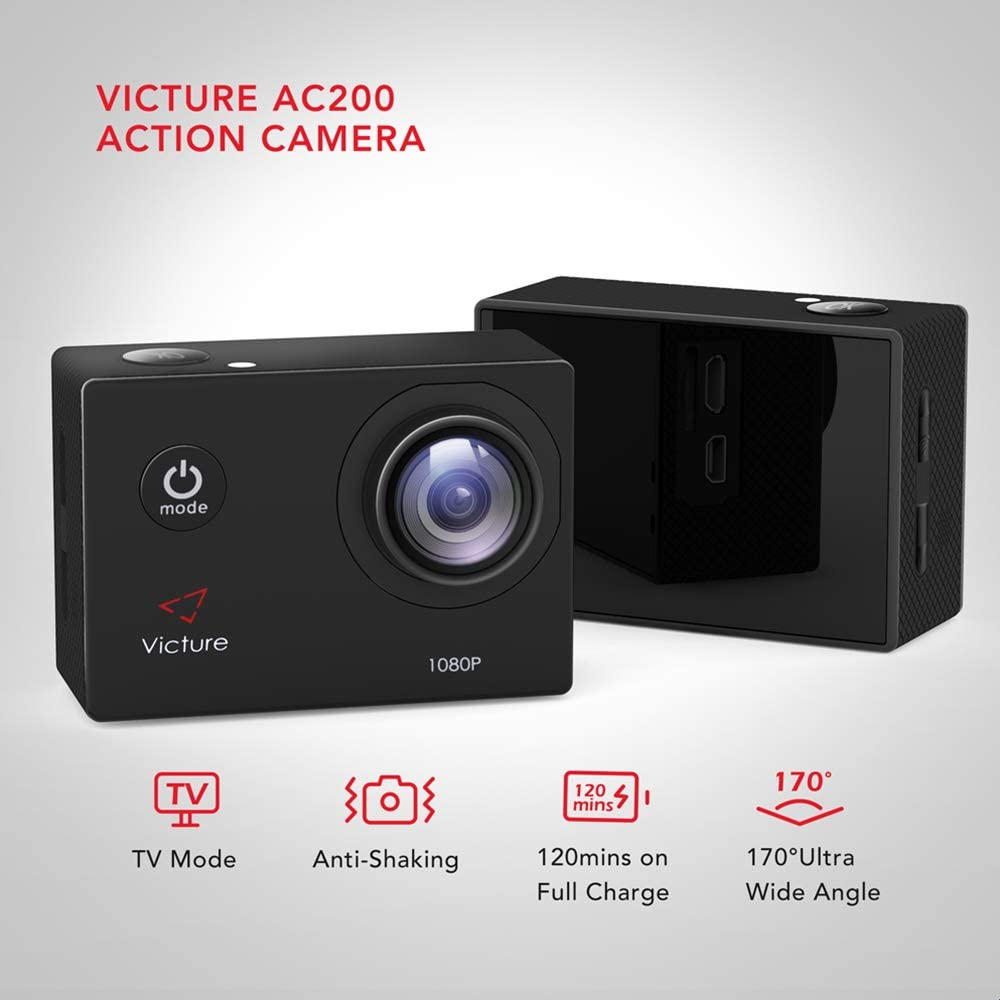
\includegraphics[width=.3\textwidth]
    {figure/equipments/victure.jpg}
    \caption{The wide angle action camera Victure AC200 that was used to record the experiments. 
    This image is copied from \cite{victure_amazon}.}
    \label{fig:victure}
\end{figure}

The choice of this particular type of camera was that a regular camera wouldn't be able to capture the 
entire stage of $\SI[product-units = single]{88.5 x 75.4}{\centi\metre}$. 
The ability of filming in a wide angle, which is a common feature in many action cameras, 
made it possible to capture the entire stage. The camera, being small and compact, made it fairly easy and practical 
to handle, especially in situations where it is needed to be removed or adjusted. 

The setup for the camera is shown in \cref{fig:table} where the camera is placed on the ground directly under the 
table. The camera needed to be fixed still at the center of the table to avoid any distortion to the footage. 

When one of the first experiments were filmed, it was clear that the lighting condition was an issue. 
The source of illumination then, was halogen lamps on the ceiling of the room which decreased the quality 
of the images significantly, see \cref{fig:bad_light}. 

\begin{figure}[htpb!]
    \centering
    %\captionsetup{justification=centering,margin=2cm}
    \includegraphics[width=.5\textwidth]
    {figure/equipments/bad_light.png}
    \caption{Low quality image as a result of bad lighting condition. Reflection of the bottom part of the wood 
    construction can be seen on the glass panel.}
    \label{fig:bad_light}
\end{figure}

To improve the quality of the footage, the lighting needed to be changed. Many configurations were tried 
out with changing the source of illumination, their placement and from which angle they should illuminate from. 
The final configuration found that gave the optimal lighting condition is shown in \cref{fig:table}. 
This setup consist of 4 spotlights placed on the floor illuminating the glass panel from 4 sides at a 
$45^{\circ}$ angle, and 9 spotlights above the table in an 3 by 3 array illuminating directly down on the 
paper sheet on top of the table. With this arrangement the quality and contrast of the image improved significantly. 
The result of this improved lighting arrangement is show in \cref{fig:good_light}, and a photograph of the lab is shown in \cref{fig:lab}.
Additional attempt were made in trying increase the contrast of bugs and obstacles against the white background, where 
the bugs body were painted black and black dots made of paper were glued under the obstacles. 

\begin{figure}[htpb!]
    \centering
    \subfloat[\label{fig:good_light}]
    {\includegraphics[width=.45\textwidth]
    {figure/equipments/good_light.png}}
    \subfloat[\label{fig:lab}]
    {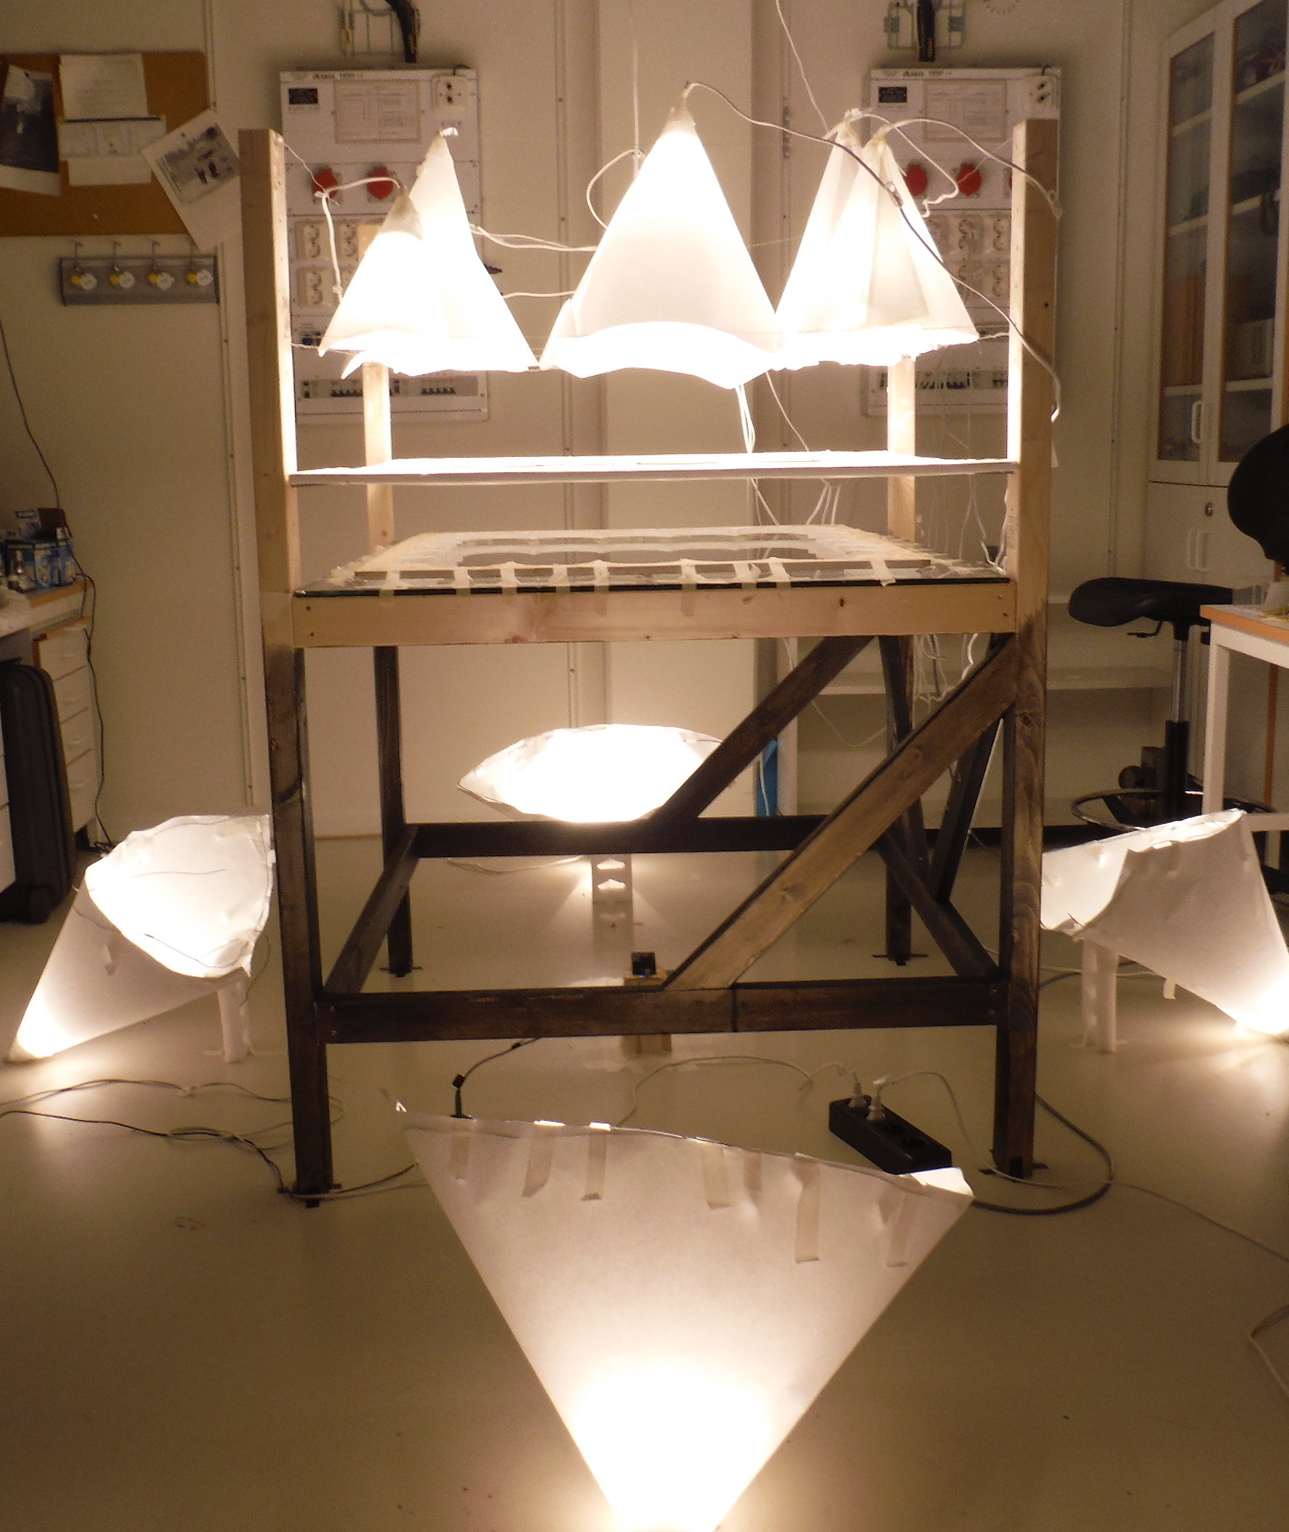
\includegraphics[width=.3\textwidth]
    {figure/equipments/lab}}
    \caption{In \textbf{(a)} an image taken with the improved lighting condition, with better quality 
    and contrast. The overview of the setup inside the lab with improved lighting is shown in \textbf{(b)}.}
    \label{fig:good_conditions}
\end{figure}


\section{The Experiment}

\subsection{How to design an experiment}

The aim of this thesis is to design a system in macroscale, consisting of active and passive particles, that 
is able to undergo a phase transition similar to the result from \cite{nilsson2017metastable}. The system 
should also show, at some condition, the behavior where the active particles form channels and reusing them.
In the simulation from \cite{nilsson2017metastable}, the collective behavior of the active particles changes 
with a noise parameter, where the active particles at a high noise level could not move far from its starting point, 
and with lower noise level they could move unhindered and forming channels in an environment of passive particles. 

Since with our robots, there is no obvious way to introduce a similar noise parameter. To recreate a similar 
conditions, we instead use the weight of the obstacles as a ''noise parameter'' where the heavier obstacles 
corresponds to the case of high noise in the simulation and lower weight obstacles corresponds low noise in the simulation. 
The number of obstacles and the number of bugs were also used as parameters. One could already guess that 
a setting with low obstacle density and low obstacle weight will lead to the bugs undergoing super-diffusive motion(moving with constant speed). 
To the opposite, having high obstacle density and high obstacle weight will lead to sub-diffusive motion with the active particles 
since their motion will be significantly impeded by the heavy obstacles.
The different variations of number of bugs $B$, number of obstacles $C$ with $W$ nuts inside, are as follows


\begin{align*}
    B &= \{1, 2, 5, 10, 15, 20, 25\} \\
    C &= \{100, 200, 300, 400, 500, 600, 700, 800, 900, 1000, 1100, 1200, 1300\} \\
    W &= \{0, 1, 2, 3\}
\end{align*}

Note that $W$ is a variable showing the number of nuts being used in each obstacles. 
The weight of a M8 nut is $m_{\text{nut}}=\SI{5}{g}$ and the weight of an empty cylinder 
is $m_{\text{cyl}}=\SI{2}{g}$. The weight of an obstacle or passive particle can then be expressed as  

\begin{align*}
    m_{\text{passive}}  =&  W(i)\cdot m_{\text{nut}} + m_{\text{cyl}} 
\end{align*}

which be eigther $\SI{2}{g}$, $\SI{7}{g}$, $\SI{12}{g}$ or $\SI{17}{g}$.
The number of experiments $N_{\text{exp}}$ that was conducted can be calculated as

\begin{align*}
    N_{\text{exp}}  &=  n(B)\times n(C)\times n(W)      \\
                    &=  364
\end{align*}    

where $n(B)$, $n(C)$ and $n(W)$ are the length of the vectors $B$, $C$ and $W$.

In addition to these, experiments without obstacles were made using 1, 2, 5, 11, 16 and 21 bugs, 
which is 6 additional experiments. This gives the total number of experiments that were made to 370.

\subsection{Conducting the experiments}

One experiment corresponds to a roughly $\unit[3]{min}$ video with a chosen number of bugs, 
obstacles and weight of the obstacles. The procedure of conducting the experiment as efficient 
as possible goes as follows


\begin{enumerate}[label*=\arabic*.]

    \item \textbf{Preparation}
    \begin{enumerate}[label*=\arabic*.]
        \item Put on the the glasspanel the chosen number of obstacles and weights and 
            spread them out as randomly as possible.
        \item Check if the batteries of the 25 bugs are good, meaning that they are not going 
        to run out after some minutes. If the batteries are to low, change it and make sure 
        to have spare bugs with enough battery power in case a bug run out of battery during an 
        experiment.
        \item Take a picture of the stage with obstacles on it and use the \MATLAB program
        \texttt{testDetection.m} to track the obstacles and see if the number is as expected.
    \end{enumerate}
    
    
    \item \textbf{Execution}
    \begin{enumerate}[label*=\arabic*.]
        \item When the preparations are done, turn on the camera and start filming.
        \item Put the first bug on the stage and let it run from time \text{0}$-$\text{3} min.
        \item Put the second bug on the stage and let it run from time \text{3}$-$\text{6} min.
        \item Put three more bugs on the stage at time \text{6} min and let in total 
            5 bugs run from time \text{6:30}$-$\text{9:30} min. The reason for letting them run 
            from \text{6:30} min instead of \text{6} min is to have a time gap for 
            checking if any bugs run out of batteries and that the stage looks ok. If there 
            is anything to be fixed, it should be done before time \text{6:30} min. 
        \item Put five more bugs on the stage at time \text{9:30} min and let in total 
            10 bugs run from time \text{10:00}$-$\text{13:00}. 
        \item Put five more bugs on the stage at time \text{13:00} min and let in total 
            15 bugs run from time \text{13:30}$-$\text{16:30} min. 
        \item Put five more bugs on the stage at time \text{16:30} min and let in total 
            20 bugs run from time \text{17:00}$-$\text{20:00} min. 
        \item At last put five more bugs on the stage at time \text{20:00} min and let in total 
            25 bugs run from time \text{20:30}$-$\text{23:30} min.
        \item One single video file of roughly \text{24} min long contains 7 experiments 
            where the number of bugs varies. When changing the number of obstacles and the 
            weight, the same procedure above is followed.
    \end{enumerate}
    
    
    \item \textbf{Postprocess}
    \begin{enumerate}[label*=\arabic*.]
        \item As mentioned above one video file contains 7 experiments. Where the number of bugs are varied.
            So to separate the different experiments, the \text{24} min video is cut and the part 
            containing a specific number of bugs is saved as separate video files. During cutting of the videos 
            it is important to remove parts of the footage that contains unwanted disturbances such 
            as shadows or hands of the experimenter, which should be removed from the footage.
            
        \item When the videos are cutted, they need to be undistorted since the 
            camera has a fish eye distortion. To achieve this, a \textsc{Matlab}\xspace program was  
            written to converting the distorted video footage 
            to image sequences where one image corresponds to one frame of the video.
        
        \item After undistortion, the image sequences are binarized, meaning changing
            the image sequences to black and white. This is for the purpose of 
            increasing the contrast between the objects that need to be tracked and 
            the background.
        
        \item When the image sequences are binarized they are tracked using two different sets 
        of codes, one for tracking the obstacles and one the bugs.
    \end{enumerate}
\end{enumerate}

The process of proceeding through the above steps for all the 370 experiments took quite 
some time. When all the steps were done, the data was save as \textsc{Matlab}\xspace structures 
holding information of the particles trajectories, orientation, also the setting of the experiment 
with the number of bugs, number of obstacles and the weight of the obstacles.
